\documentclass{amsbook}

\usepackage{../HBSuerDemir}

\graphicspath{{images/}}

\begin{document}

\hPage{b1p2/364}

\begin{thm}
	The area $\hAbs{R}$ of the plane region R bounded by the curve y = f(x), x-axis and the vertical lines x = a, x = b 	is given by \\
	\begin{equation*}
		\hAbs{R} = \int_{a}^{b} \! \hAbs{f(x)} \, \hDif x \quad (f(x) \in C(a,\ b))
	\end{equation*} \\
\end{thm}

\begin{proof} 
	The statement is trivially true if $f(x) > 0$ on $(a,\ b)$, since the RIEMANN sum \\
	\begin{equation*}
		\sum_{i = 1}^{n} f(t_i) \Delta{x_i}
	\end{equation*} \\ \\
	is an approximation of the area under the curve and the limit is the area $\hAbs{R}$. (See left fig.) \\
\end{proof}

\noindent 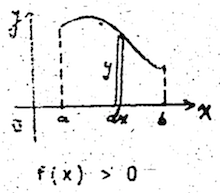
\includegraphics{1} 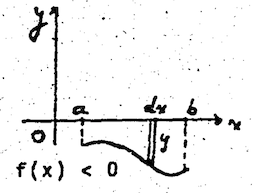
\includegraphics{2} 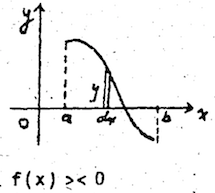
\includegraphics{3} \\

If $f(x) < 0$ on $(a,\ b)$, we have
\begin{equation*}
	\hAbs{R} = \int_{a}^{b} \! (-f(x)) \, \hDif x = \int_{a}^{b} \! \hAbs{f(x)} \, \hDif x
\end{equation*}

If $f(x)$ is positive and negative on $(a,\ b)$, say positive on $(a,\ x_0)$, and negative on $(x_0,\ b)$, then one gets
\begin{align*}
	\hAbs{R} &= \int_{a}^{x_0} \! f(x) \, \hDif x + \int_{x_0}^{b} \! (-f(x)) \, \hDif x \\
	&= \int_{a}^{x_0} \! \hAbs{f(x)} \, \hDif x + \int_{x_0}^{b} \! \hAbs{f(x)} \, \hDif x = \int_{a}^{b} \! \hAbs{f(x)} \, \hDif x
\end{align*}

\begin{cor}
	The area of a plane region bounded by the curve y = f(x), the y-axis and the horizontal lines y = c, y = d is 		given by
\end{cor}

\thispagestyle{empty} 
\end{document} 